\documentclass{../../slides-style}

\usepackage{algpseudocode}

\slidetitle{Разбор контрольной}{21.03.2026}

\begin{document}
    
    \begin{frame}[plain]
        \titlepage
    \end{frame}

    \begin{frame}{Разбор летучки}
        Задача 1, про матрицу инцидентности
        $$
        M = \begin{pmatrix}
        1 & 0 & 0 & 0 & -1 \\
        -1 & -1 & 1 & 0 & 0 \\
        0 & 0 & -1 & -1 & 0 \\
        0 & 1 & 0 & 1 & 1
        \end{pmatrix}
        $$
        \begin{center}
            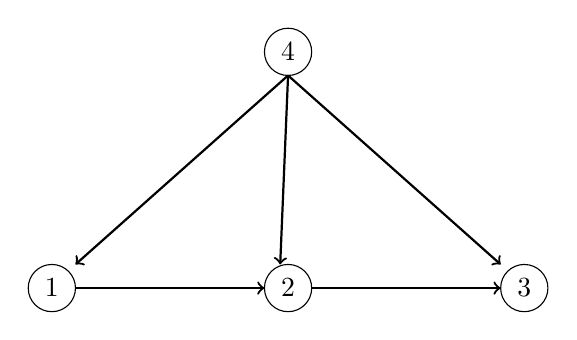
\begin{tikzpicture}
                \draw (0,0) circle (0.3cm) node {1};
                \draw (3,0) circle (0.3cm) node {2};
                \draw (6,0) circle (0.3cm) node {3};
                \draw (3,3) circle (0.3cm) node {4};

                \draw[->, thick] (0.3,0) -- (2.7,0);

                \draw[->, thick] (3.3,0) -- (5.7,0);

                \draw[->, thick] (3,2.7) -- (0.3,0.3);
                \draw[->, thick] (3,2.7) -- (2.9,0.3);
                \draw[->, thick] (3,2.7) -- (5.7,0.3);
            \end{tikzpicture}
        \end{center}
    \end{frame}

    \begin{frame}{Разбор летучки}
        Задача 2, про трудоёмкость BFS в худшем случае
        \begin{outline}
            \1 $O(|V| + |E|)$
            \1 BFS запоминает посещённые вершины и посещает каждую ровно один раз, но должен просмотреть все рёбра от каждой вершины
            \1 Худший случай --- если граф полносвязный и надо обойти его весь, трудоёмкость такая же
                \1 $|E| \in O(|V|^2)$, так что общая трудоёмкость получится $O(|V|^2)$, что не противоречит написанному выше
            \1 Ответ без пояснений полностью не засчитывался
        \end{outline}
    \end{frame}

    \begin{frame}[fragile]{Разбор летучки}
        Задача 3, про функцию neighbours
        \begin{minted}{c}
void neighbours(int v, int size, int** graph) {
    if (v < 0 || v >= size || graph == NULL || *graph == NULL) {
        return;
    }

    for (int i = 0; i < size; ++i) {
        if (graph[v][i]) {
            printf("%d ", i);
        }
    }
}
        \end{minted}
    \end{frame}

    \begin{frame}{Разбор контрольной}
        Задача 1, АВЛ-дерево
        \begin{center}
            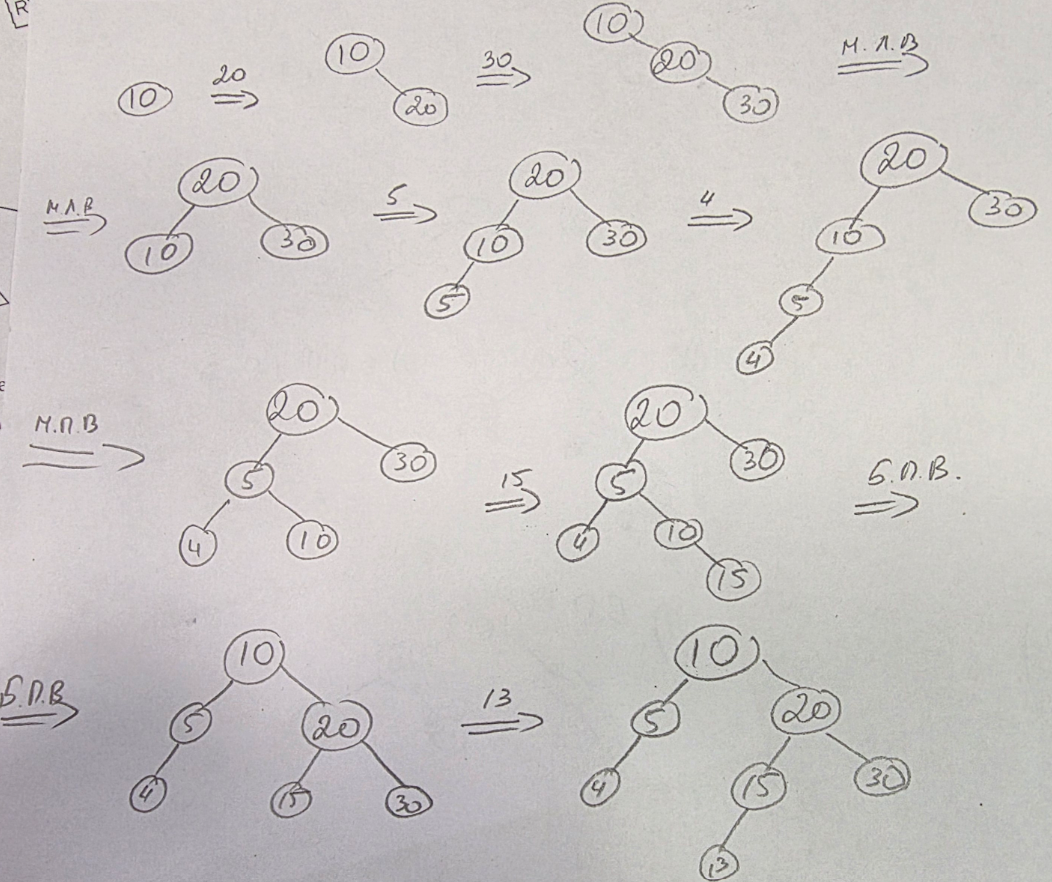
\includegraphics[height=0.8\textheight]{avl.png}
        \end{center}
    \end{frame}

    \begin{frame}{Разбор контрольной}
        \framesubtitle{Задача 2, Дейкстра}
        Матрица смежности:
        \begin{center}
            $$
            \begin{pmatrix}
            & 1 & 2 & 3 & 4 \\
            1 & - & 3 & 1 & - \\
            2 & - & - & - & 2 \\
            3 & - & 1 & - & 5 \\
            4 & - & - & - & -
            \end{pmatrix}
            $$
        \end{center}
        Визуализация графа:
        \begin{center}
            
\includegraphics[width=0.6\textwidth]{graph.png}
        \end{center}
    \end{frame}

    \begin{frame}{Разбор контрольной}
        \framesubtitle{Задача 2, Дейкстра}
        Таблица:
        \begin{center}
            \begin{tabu}{c c c c c c}
                \hline
                Шаг    & Текущая вершина & d[1] & d[2]  & d[3]  & d[4]  \\
                \hline
                Начало & —               &    0 &     ∞ &    ∞  &    ∞  \\
                1      & 1               &    0 & 3 (1) & 1 (1) &    ∞  \\
                2      & 3               &    0 & 2 (3) & 1 (1) & 6 (3) \\
                3      & 2               &    0 & 2 (3) & 1 (1) & 4 (2) \\
                4      & 4               &    0 & 2 (3) & 1 (1) & 4 (2) \\
                \hline
            \end{tabu}
        \end{center}
        Путь: $1 \rightarrow 3 \rightarrow 2 \rightarrow 4$, длина 4
    \end{frame}

    \begin{frame}{Разбор контрольной}
        \framesubtitle{Задача 2, Дейкстра}
        Проблемы:
        \begin{outline}
            \1 Многие забыли указать путь и/или длину пути
            \1 На шаге 2 в d[4] оказывались значения от 5 до 8
        \end{outline}
    \end{frame}

    \begin{frame}[fragile]{Разбор контрольной}
        \framesubtitle{Задача 3, высота узла}
        \begin{footnotesize}
            \begin{minted}{c}
int nodeHeight(Node *root, int key) {
    if (root == NULL) return -1;

    if (key < root->key)
        return nodeHeight(root->left, key);
    if (key > root->key)
        return nodeHeight(root->right, key);

    return height(root);
}

int height(Node *node) {
    if (node == NULL) return -1;
    int leftH  = height(node->left);
    int rightH = height(node->right);
    return (leftH > rightH ? leftH : rightH) + 1;
}
            \end{minted}
        \end{footnotesize}
    \end{frame}

    \begin{frame}[fragile]{Разбор контрольной}
        \framesubtitle{Задача 3, высота узла}
        Ещё одно решение, без вспомогательной функции:
        \begin{footnotesize}
            \begin{minted}{c}
int nodeHeight(Node *root, int key) {
    if (root == NULL) return -1;

    if (key < root->key)
        return nodeHeight(root->left, key);
    if (key > root->key)
        return nodeHeight(root->right, key);

    int leftH  = node->left ? nodeHeight(node->left, node->left->key) : -1;
    int rightH = node->right ? nodeHeight(node->right, node->right->key) : -1;
    return (leftH > rightH ? leftH : rightH) + 1;
}
            \end{minted}
        \end{footnotesize}
    \end{frame}

    \begin{frame}{Разбор контрольной}
        \framesubtitle{Задача 4, сложность Дейкстры}
        \begin{outline}
            \1 Наивная реализация: $O(|V|^2 + |E|)$ = $O(|V|^2)$, --- мы при посещении каждой вершины ищем ближайшую к стартовой за линию (граф может быть полносвязным) и обновляем длины путей, проходясь по рёбрам (не более одного раза каждое)
            \1 С кучей: $O(|V|log(|V|) + |E|log(|V|))$ --- извлечение минимума из кучи за логарифм, обновление расстояния за логарифм (вставка в кучу) для каждого исходящего ребра (всего $|E|$ раз)
            \1 Многие написали ответ, но не пояснили, почему
            \1 Многие забыли про рёбра
        \end{outline}
    \end{frame}

    \begin{frame}{Разбор контрольной}
        \framesubtitle{Задача 5, умножение матриц}
        \begin{enumerate}
            \item[a)] Массивы хранятся в row-major порядке: B[k][0], B[k][1], \dots лежат подряд, B[0][j], B[1][j], \dots --- вразброс, так что в matmul\_v1 (где обход B в column-major) происходят промахи кеша. В matmul\_v2 все матрицы читаются в row-major, кеш используется максимально
            \item[b)] Кеш-линии обычно 64 байта, при последовательном доступе одно чтение на 16 значений из матрицы, при column-major --- на одно
            \item[c)] Проверить можно \mintinline{bash}|perf stat -e cache-misses,cache-references ./matmul_v1| (или matmul\_v2)
        \end{enumerate}
        \begin{outline}
            \1 Требовалось внятное объяснение, хотя бы упоминающее кеш и последовательность доступа
            \1 Никто не ожидал ключи для perf, но надо было написать, что именно смотреть для проверки гипотезы
        \end{outline}
    \end{frame}

\end{document}